\documentclass[11pt]{article}

% Packages
\usepackage[margin=1in, top=0.7in]{geometry}
\usepackage{amsmath,amssymb,amsfonts}
\usepackage{graphicx}
\graphicspath{{./}{../}}
\usepackage{hyperref}
\usepackage{algorithm}
\usepackage{algpseudocode}
\usepackage{booktabs}
\usepackage{longtable}
\usepackage{multirow}

% Document info
\title{Assignment 2 Report\\
    CS-726: Advanced Machine Learning}
\author{Deeptanshu Malu \quad Deevyanshu Malu \quad Neel Rambhia}
\date{}

\begin{document}

\maketitle

\section{Denoising Diffusion Probabilistic Models}
For NLL caluclation, the temperature is set to 0.1.
For EMD calculation, the number of subsamples is set to 250 and the number of iterations is set to 5.

\subsection{Varying Timesteps}
Here, lbeta = 0.0001 and ubeta = 0.02.

\begin{longtable}{|l|l|c|c|c|c|c|c|}
    \hline
    \textbf{Dataset} & \textbf{Metric} & \multicolumn{6}{c|}{\textbf{Timesteps}} \\
    \cline{3-8}
    & & \textbf{10} & \textbf{50} & \textbf{100} & \textbf{150} & \textbf{200} & \textbf{500} \\
    \hline
    \multirow{2}{*}{Moons} & EMD & 39.99 & 28.95 & \textbf{27.40} & 29.64 & 30.55 & 44.90 \\
    \cline{2-8}
    & NLL & 1.02 & 0.96 & 0.94 & \textbf{0.93} & 0.94 & 0.95 \\
    \hline
    \multirow{2}{*}{Circles} & EMD & 34.60 & \textbf{31.48} & 33.24 & 34.41 & 38.62 & 42.04 \\
    \cline{2-8}
    & NLL & 1.05 & 0.99 & 1.00 & \textbf{0.98} & 1.01 & 1.03 \\
    \hline
    \multirow{2}{*}{Blobs} & EMD & 88.78 & 43.69 & 20.08 & 18.36 & \textbf{17.17} & 19.83 \\
    \cline{2-8}
    & NLL & 0.34 & 0.12 & 0.04 & 0.03 & \textbf{0.01} & 0.04 \\
    \hline
    \multirow{2}{*}{Manycircles} & EMD & 33.65 & \textbf{26.41} & 27.77 & 27.98 & 30.98 & 30.34 \\
    \cline{2-8}
    & NLL & 0.66 & \textbf{0.54} & 0.54 & 0.54 & 0.54 & 0.58 \\
    \hline
    \multirow{2}{*}{Helix} & EMD & 56.00 & 59.33 & 57.15 & \textbf{56.13} & 58.87 & 60.49 \\
    \cline{2-8}
    & NLL & 1.55 & 1.53 & 1.52 & 1.52 & 1.53 & \textbf{1.51} \\
    \hline
\end{longtable}

\begin{figure}[ht]
    \centering
    \begin{tabular}{ccc}
        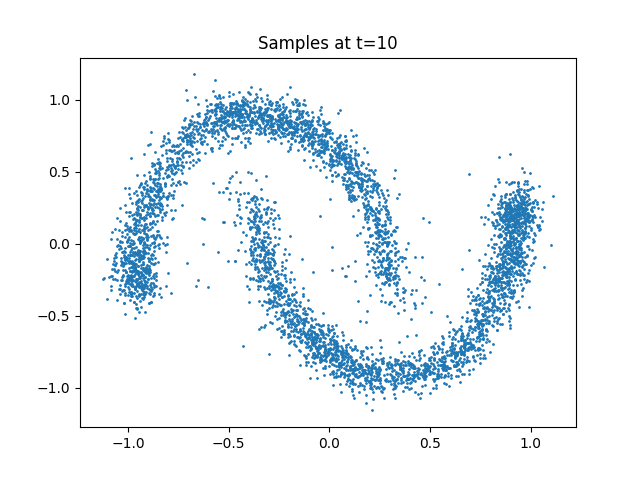
\includegraphics[width=0.3\textwidth]{exps/ddpm_2_10_0.0001_0.02_moons/samples_10.png} &
        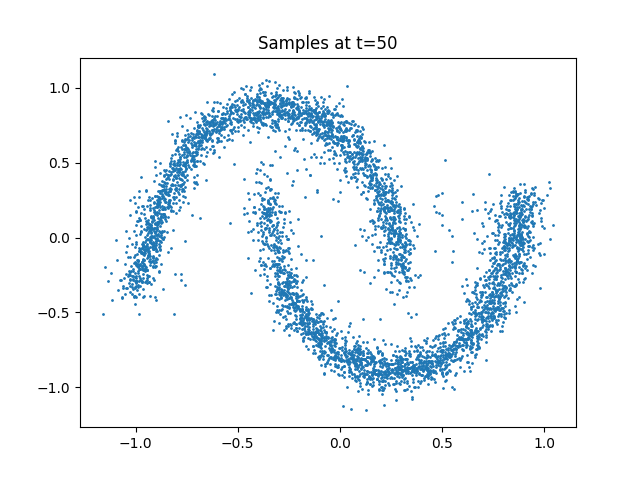
\includegraphics[width=0.3\textwidth]{exps/ddpm_2_50_0.0001_0.02_moons/samples_50.png} &
        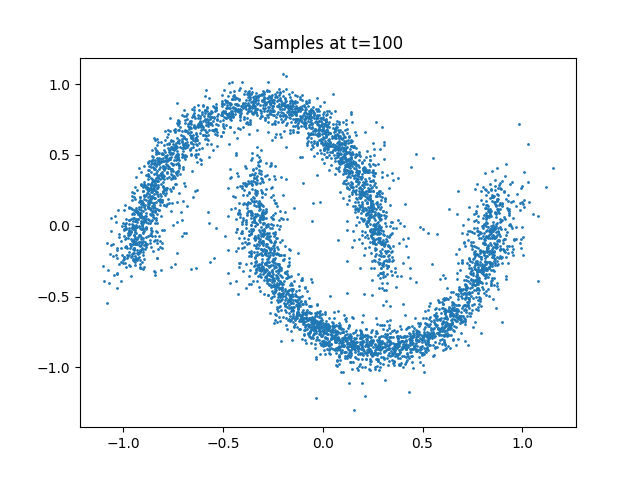
\includegraphics[width=0.3\textwidth]{exps/ddpm_2_100_0.0001_0.02_moons/samples_100.png} \\
        t=10 & t=50 & t=100 \\[0.5em]
        
        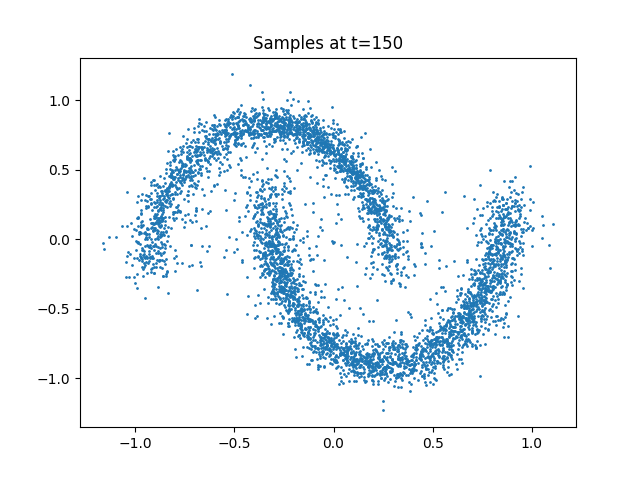
\includegraphics[width=0.3\textwidth]{exps/ddpm_2_150_0.0001_0.02_moons/samples_150.png} &
        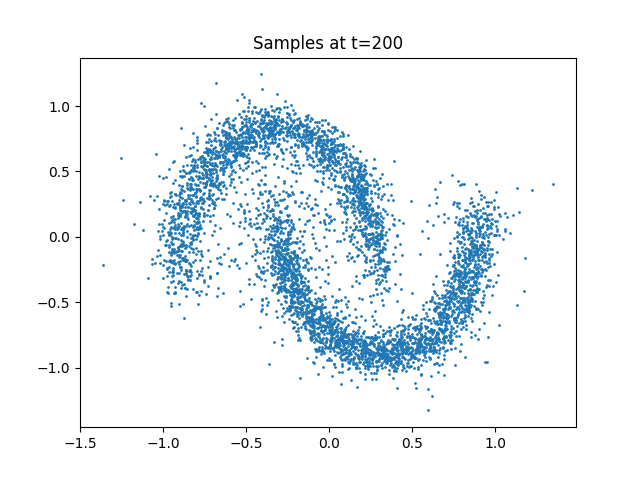
\includegraphics[width=0.3\textwidth]{exps/ddpm_2_200_0.0001_0.02_moons/samples_200.png} &
        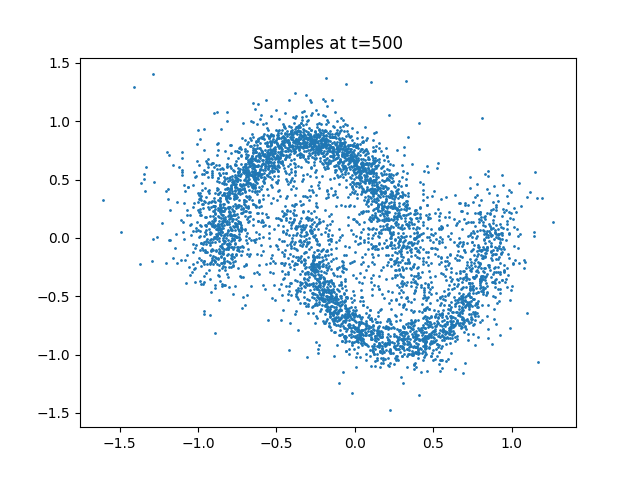
\includegraphics[width=0.3\textwidth]{exps/ddpm_2_500_0.0001_0.02_moons/samples_500.png} \\
        t=150 & t=200 & t=500 \\
    \end{tabular}
    \caption{Samples generated by DDPM with \textbf{varying timesteps} for the Moons dataset.}
    \label{fig:timesteps_moons}
\end{figure}

\begin{figure}[ht]
    \centering
    \begin{tabular}{ccc}
        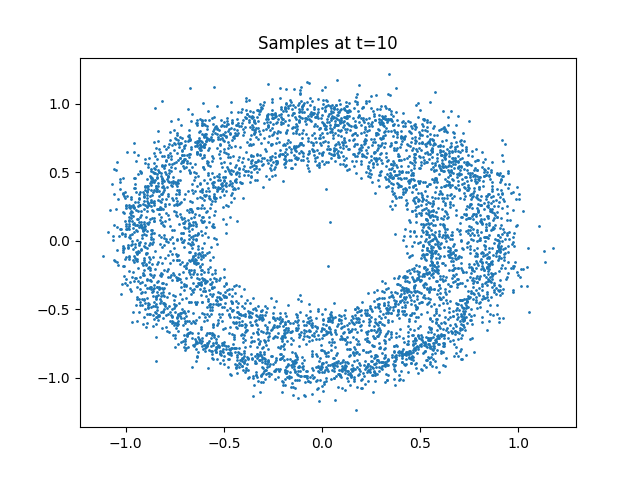
\includegraphics[width=0.3\textwidth]{exps/ddpm_2_10_0.0001_0.02_circles/samples_10.png} &
        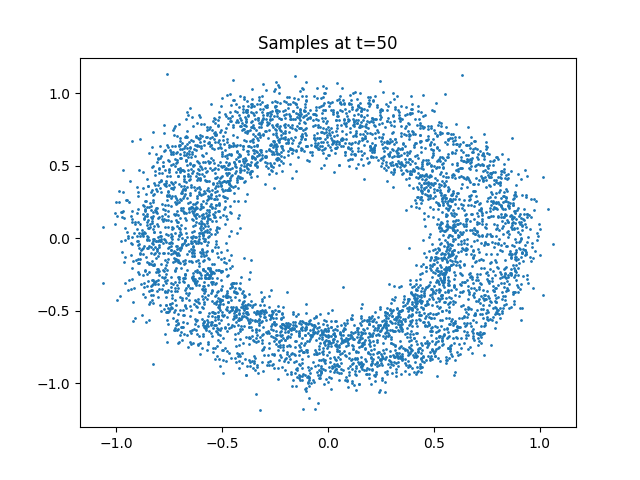
\includegraphics[width=0.3\textwidth]{exps/ddpm_2_50_0.0001_0.02_circles/samples_50.png} &
        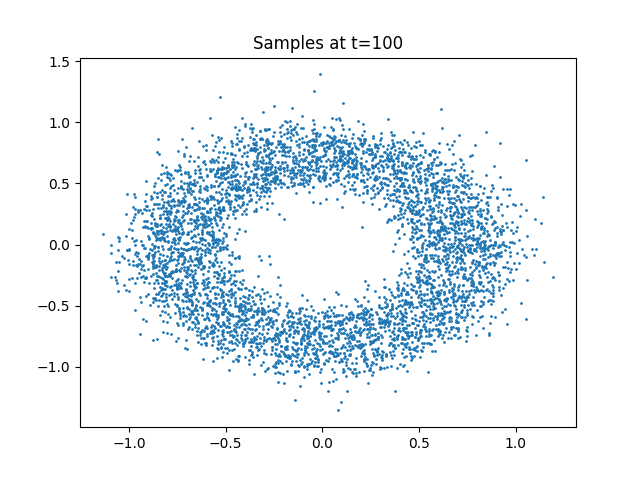
\includegraphics[width=0.3\textwidth]{exps/ddpm_2_100_0.0001_0.02_circles/samples_100.png} \\
        t=10 & t=50 & t=100 \\[0.5em]
        
        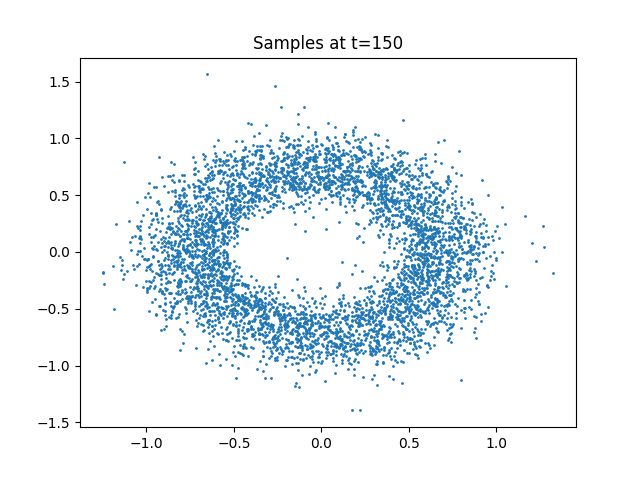
\includegraphics[width=0.3\textwidth]{exps/ddpm_2_150_0.0001_0.02_circles/samples_150.png} &
        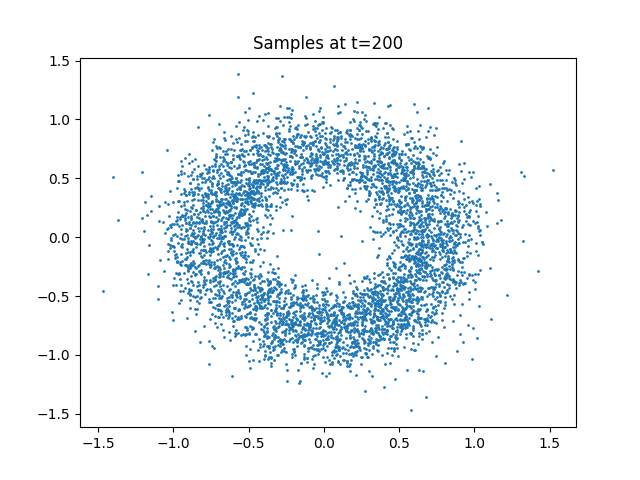
\includegraphics[width=0.3\textwidth]{exps/ddpm_2_200_0.0001_0.02_circles/samples_200.png} &
        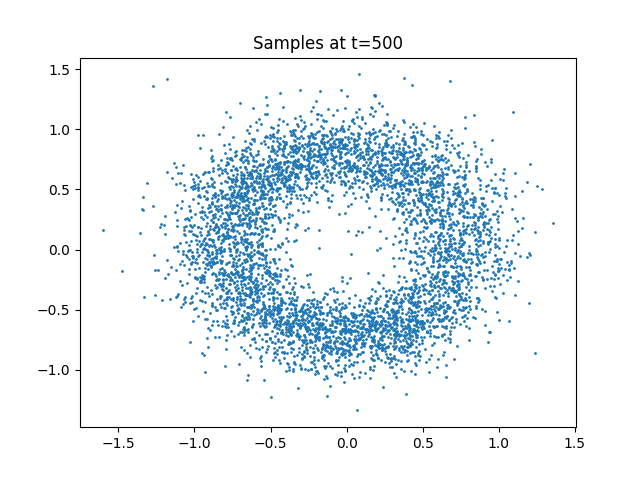
\includegraphics[width=0.3\textwidth]{exps/ddpm_2_500_0.0001_0.02_circles/samples_500.png} \\
        t=150 & t=200 & t=500 \\
    \end{tabular}
    \caption{Samples generated by DDPM with \textbf{varying timesteps} for the Circles dataset.}
    \label{fig:timesteps_circles}
\end{figure}

\begin{figure}[ht]
    \centering
    \begin{tabular}{ccc}
        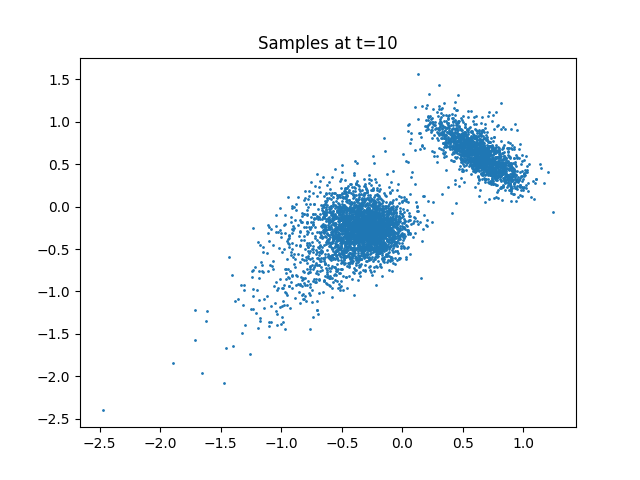
\includegraphics[width=0.3\textwidth]{exps/ddpm_2_10_0.0001_0.02_blobs/samples_10.png} &
        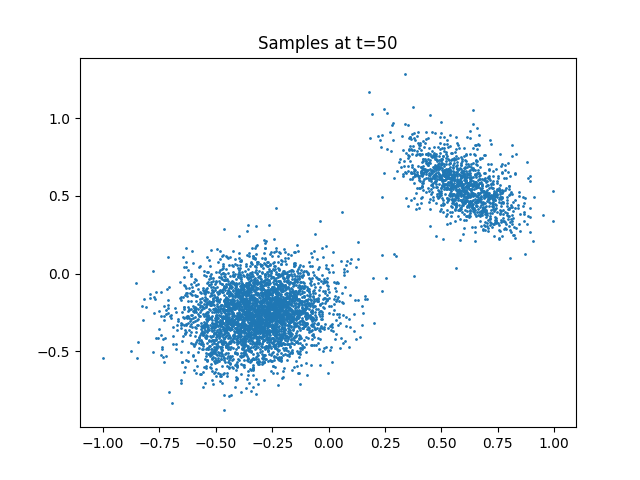
\includegraphics[width=0.3\textwidth]{exps/ddpm_2_50_0.0001_0.02_blobs/samples_50.png} &
        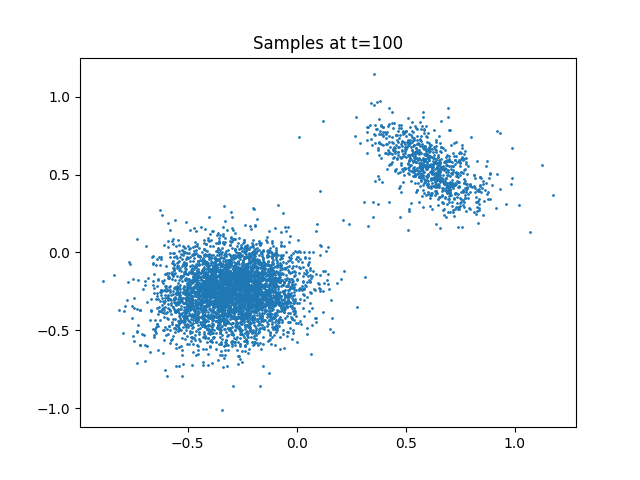
\includegraphics[width=0.3\textwidth]{exps/ddpm_2_100_0.0001_0.02_blobs/samples_100.png} \\
        t=10 & t=50 & t=100 \\[0.5em]
        
        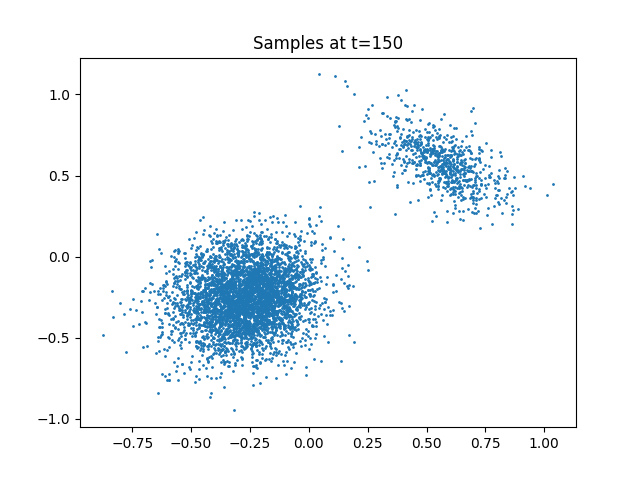
\includegraphics[width=0.3\textwidth]{exps/ddpm_2_150_0.0001_0.02_blobs/samples_150.png} &
        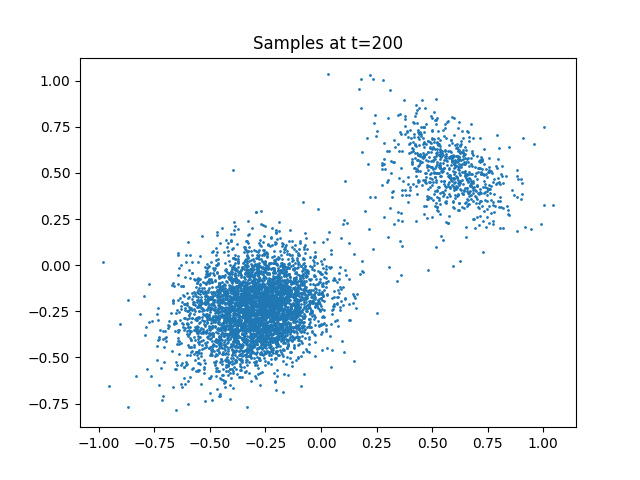
\includegraphics[width=0.3\textwidth]{exps/ddpm_2_200_0.0001_0.02_blobs/samples_200.png} &
        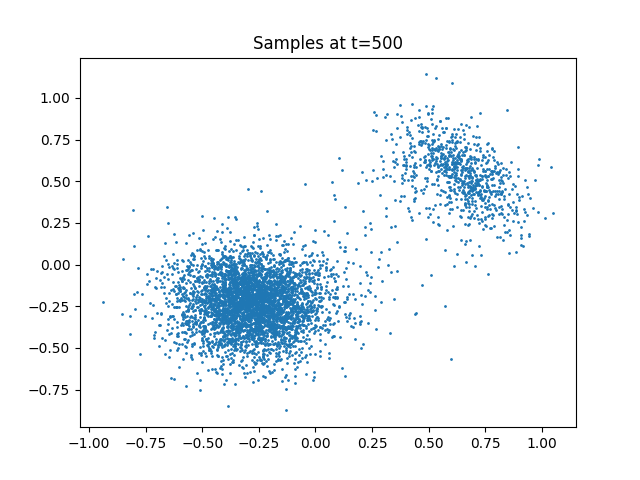
\includegraphics[width=0.3\textwidth]{exps/ddpm_2_500_0.0001_0.02_blobs/samples_500.png} \\
        t=150 & t=200 & t=500 \\
    \end{tabular}
    \caption{Samples generated by DDPM with \textbf{varying timesteps} for the Blobs dataset.}
    \label{fig:timesteps_blobs}
\end{figure}

\begin{figure}[ht]
    \centering
    \begin{tabular}{ccc}
        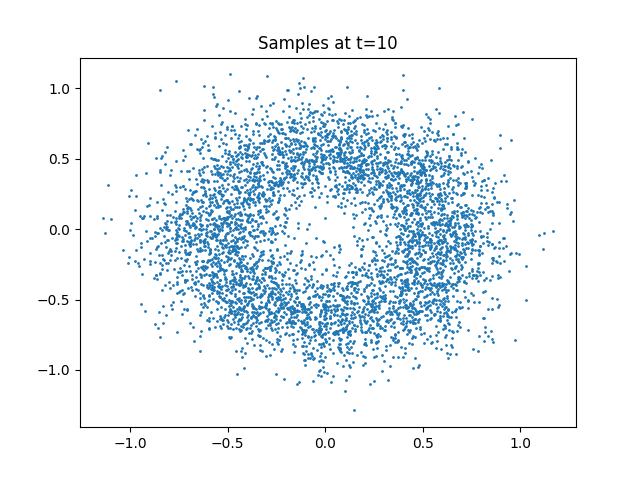
\includegraphics[width=0.3\textwidth]{exps/ddpm_2_10_0.0001_0.02_manycircles/samples_10.png} &
        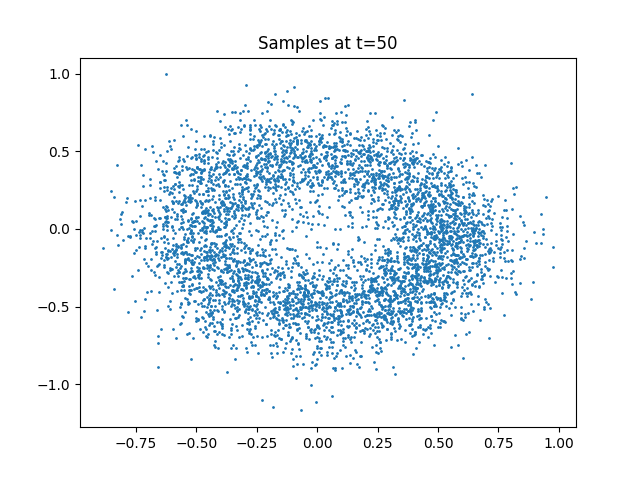
\includegraphics[width=0.3\textwidth]{exps/ddpm_2_50_0.0001_0.02_manycircles/samples_50.png} &
        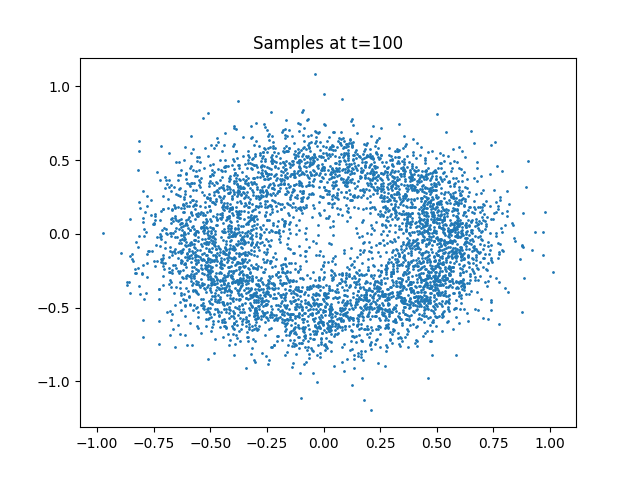
\includegraphics[width=0.3\textwidth]{exps/ddpm_2_100_0.0001_0.02_manycircles/samples_100.png} \\
        t=10 & t=50 & t=100 \\[0.5em]
        
        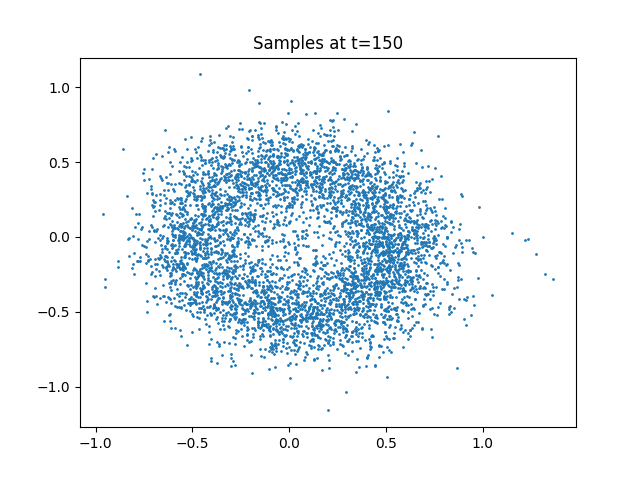
\includegraphics[width=0.3\textwidth]{exps/ddpm_2_150_0.0001_0.02_manycircles/samples_150.png} &
        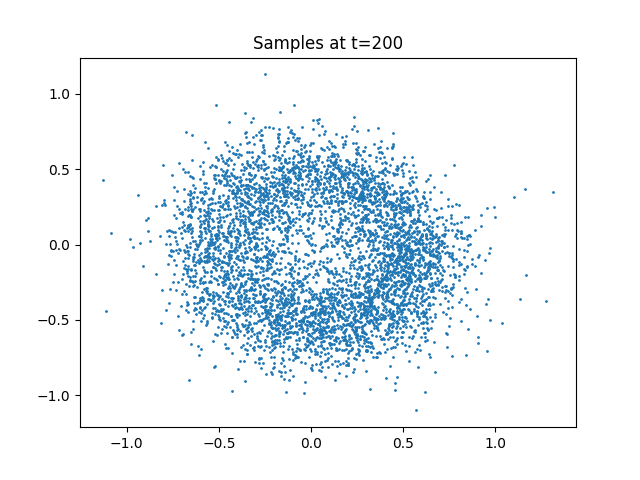
\includegraphics[width=0.3\textwidth]{exps/ddpm_2_200_0.0001_0.02_manycircles/samples_200.png} &
        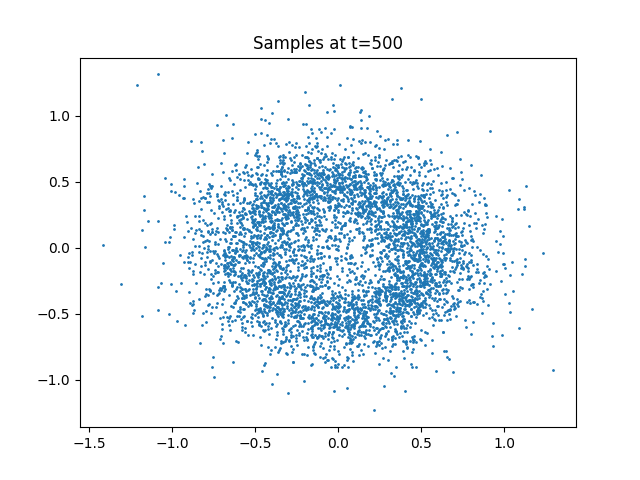
\includegraphics[width=0.3\textwidth]{exps/ddpm_2_500_0.0001_0.02_manycircles/samples_500.png} \\
        t=150 & t=200 & t=500 \\
    \end{tabular}
    \caption{Samples generated by DDPM with \textbf{varying timesteps} for the Manycircles dataset.}
    \label{fig:timesteps_manycircles}
\end{figure}

\begin{figure}[ht]
    \centering
    \begin{tabular}{ccc}
        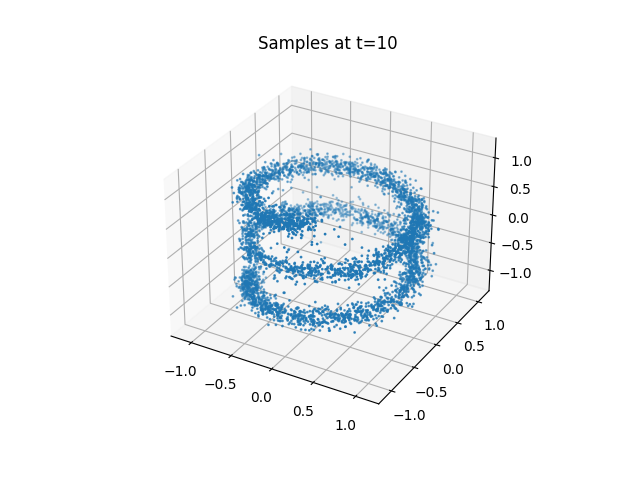
\includegraphics[width=0.3\textwidth]{exps/ddpm_3_10_0.0001_0.02_helix/samples_10.png} &
        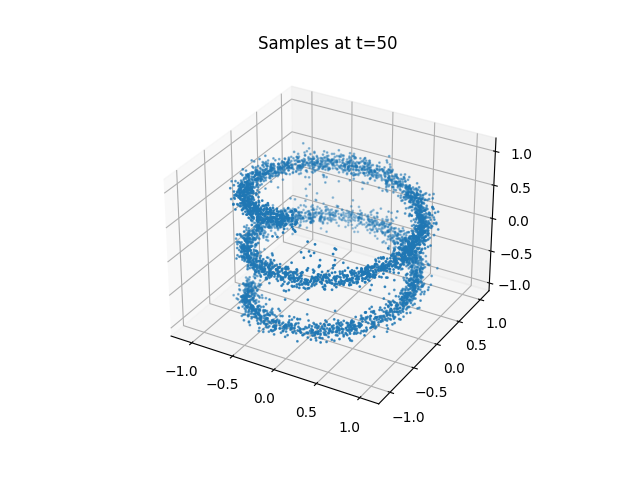
\includegraphics[width=0.3\textwidth]{exps/ddpm_3_50_0.0001_0.02_helix/samples_50.png} &
        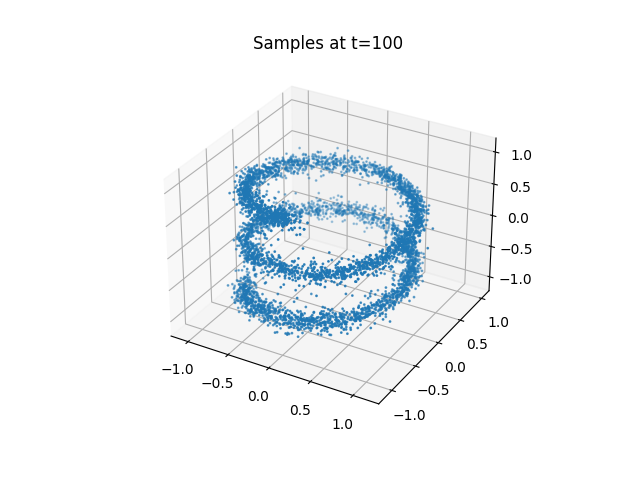
\includegraphics[width=0.3\textwidth]{exps/ddpm_3_100_0.0001_0.02_helix/samples_100.png} \\
        t=10 & t=50 & t=100 \\[0.5em]
        
        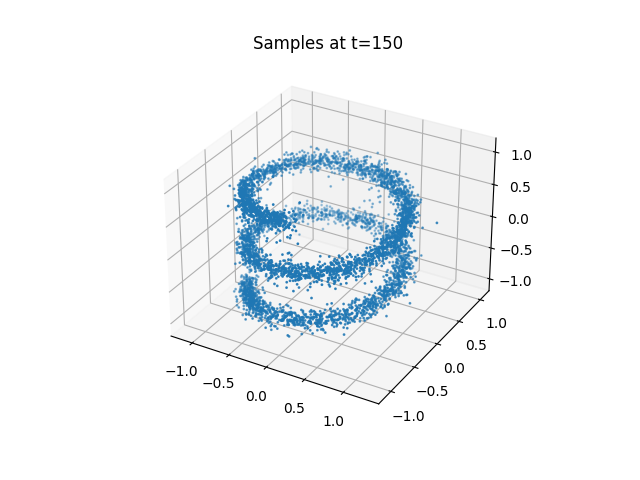
\includegraphics[width=0.3\textwidth]{exps/ddpm_3_150_0.0001_0.02_helix/samples_150.png} &
        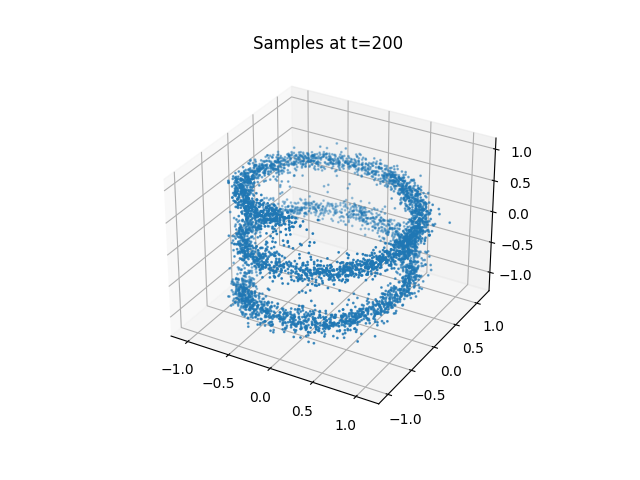
\includegraphics[width=0.3\textwidth]{exps/ddpm_3_200_0.0001_0.02_helix/samples_200.png} &
        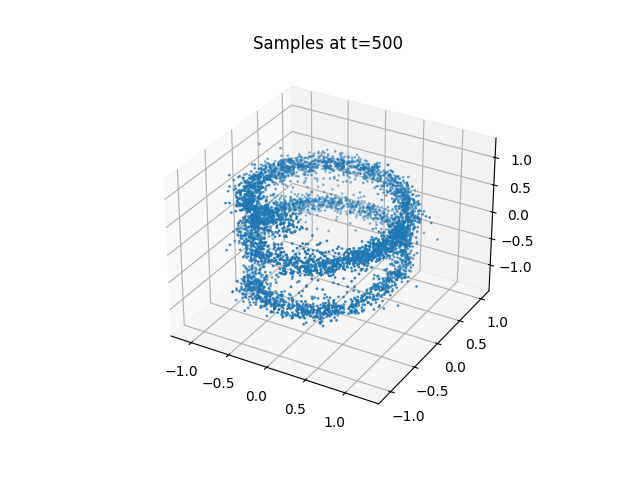
\includegraphics[width=0.3\textwidth]{exps/ddpm_3_500_0.0001_0.02_helix/samples_500.png} \\
        t=150 & t=200 & t=500 \\
    \end{tabular}
    \caption{Samples generated by DDPM with \textbf{varying timesteps} for the Helix dataset.}
    \label{fig:timesteps_helix}
\end{figure}

\subsection{Varying Beta Schedule}
Here, timesteps = 200.

\begin{longtable}{|l|l|c|c|c|c|c|c|}
    \hline
     \textbf{Dataset} & \textbf{Metric} & \multicolumn{6}{c|}{\textbf{Beta Schedule (lbeta→ubeta)}} \\
     \cline{3-8}
     & & \textbf{1e-4→0.02} & \textbf{1e-3→0.2} & \textbf{1e-5→0.002} & \textbf{1e-5→0.02} & \textbf{1e-4→0.2} & \textbf{1e-5→0.2} \\
    \hline
        \multirow{2}{*}{Moons} & EMD & 30.55 & 35.57 & 34.76 & \textbf{30.48} & 33.48 & 33.62 \\
        \cline{2-8}
        & NLL & 0.94 & \textbf{0.93} & 0.98 & 0.95 & 0.95 & 0.94 \\
        \hline
        \multirow{2}{*}{Circles} & EMD & 38.62 & 38.03 & \textbf{33.03} & 38.36 & 36.52 & 37.45 \\
        \cline{2-8}
        & NLL & 1.01 & \textbf{1.00} & 1.02 & \textbf{1.00} & 1.01 & 1.01 \\
        \hline
        \multirow{2}{*}{Blobs} & EMD & \textbf{17.17} & 20.35 & 62.98 & \textbf{17.17} & 19.59 & 19.62 \\
        \cline{2-8}
        & NLL & 0.01 & 0.02 & 0.20 & 0.01 & 0.01 & \textbf{0.00} \\
        \hline
        \multirow{2}{*}{Manycircles} & EMD & 30.98 & 28.75 & \textbf{26.55} & 31.82 & 29.40 & 29.92 \\
        \cline{2-8}
        & NLL & 0.54 & \textbf{0.52} & 0.58 & 0.53 & 0.53 & 0.54 \\
        \hline
        \multirow{2}{*}{Helix} & EMD & 58.87 & \textbf{56.25} & 57.31 & 58.29 & 57.34 & 58.72 \\
        \cline{2-8}
        & NLL & 1.53 & \textbf{1.52} & 1.54 & 1.53 & 1.53 & 1.52 \\
        \hline
    \end{longtable}

    \begin{figure}[ht]
        \centering
        \begin{tabular}{ccc}
            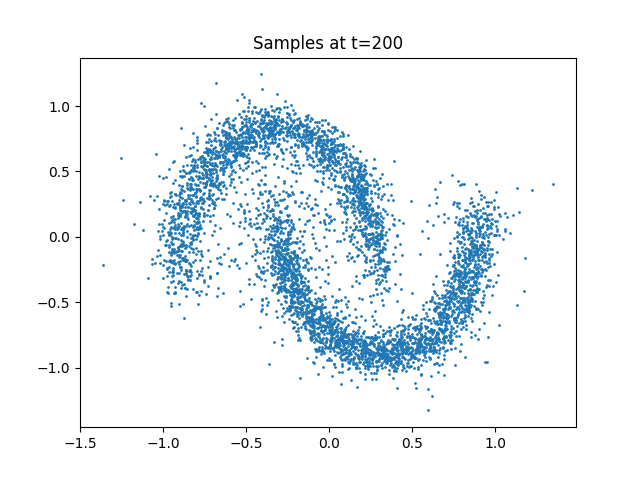
\includegraphics[width=0.3\textwidth]{exps/ddpm_2_200_0.0001_0.02_moons/samples_200.png} &
            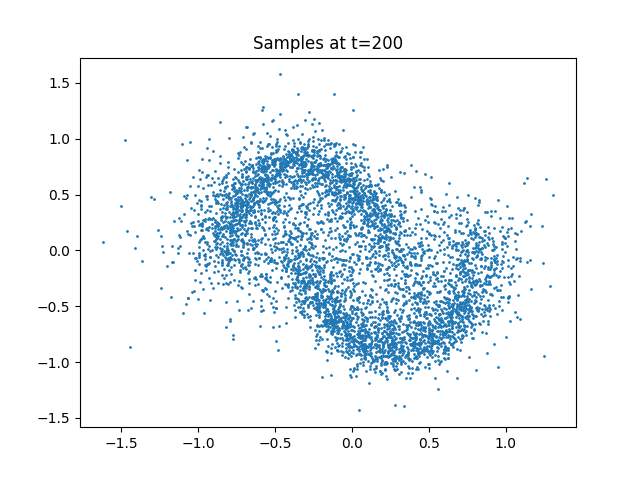
\includegraphics[width=0.3\textwidth]{exps/ddpm_2_200_0.001_0.2_moons/samples_200.png} &
            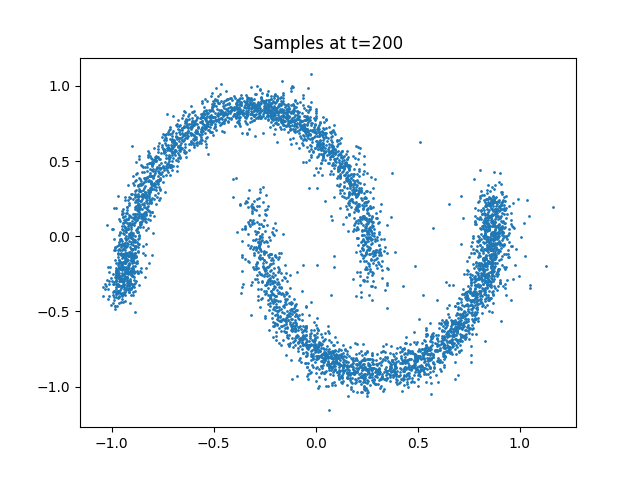
\includegraphics[width=0.3\textwidth]{exps/ddpm_2_200_1e-05_0.002_moons/samples_200.png} \\
            $\beta=1\text{e-}4\to0.02$ & $\beta=1\text{e-}3\to0.2$ & $\beta=1\text{e-}5\to0.002$ \\[0.5em]
            
            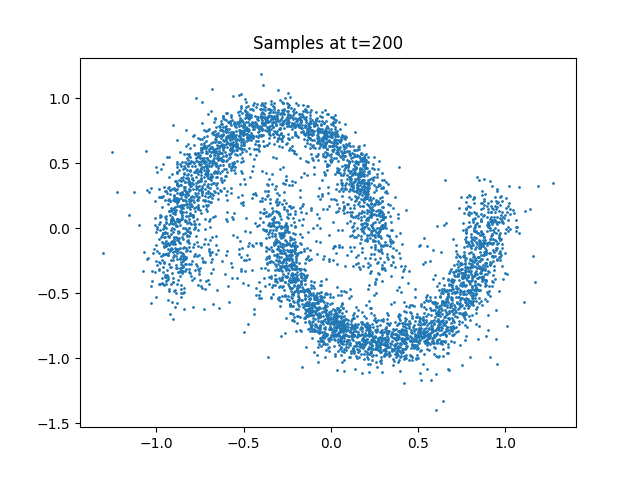
\includegraphics[width=0.3\textwidth]{exps/ddpm_2_200_1e-05_0.02_moons/samples_200.png} &
            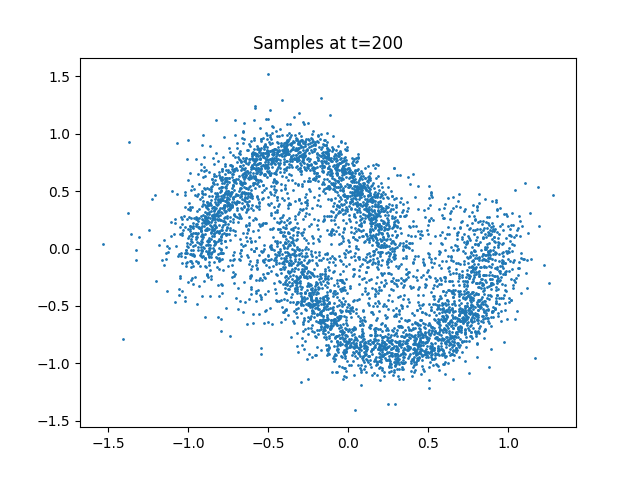
\includegraphics[width=0.3\textwidth]{exps/ddpm_2_200_0.0001_0.2_moons/samples_200.png} &
            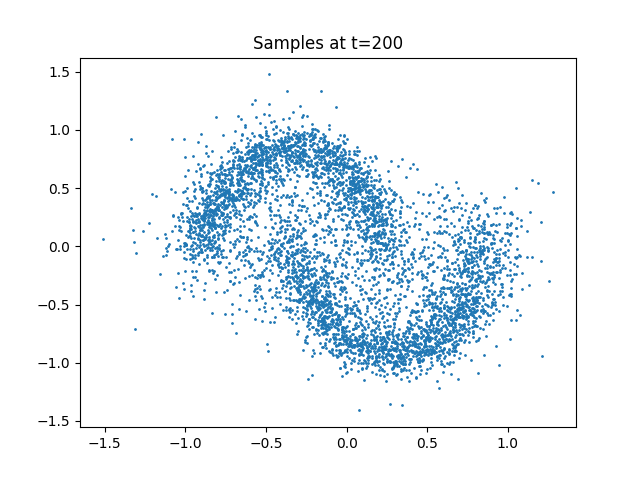
\includegraphics[width=0.3\textwidth]{exps/ddpm_2_200_1e-05_0.2_moons/samples_200.png} \\
            $\beta=1\text{e-}5\to0.02$ & $\beta=1\text{e-}4\to0.2$ & $\beta=1\text{e-}5\to0.2$ \\
        \end{tabular}
        \caption{Samples generated by DDPM with \textbf{varying beta schedules} for the Moons dataset.}
        \label{fig:beta_moons}
    \end{figure}

    \begin{figure}[ht]
        \centering
        \begin{tabular}{ccc}
            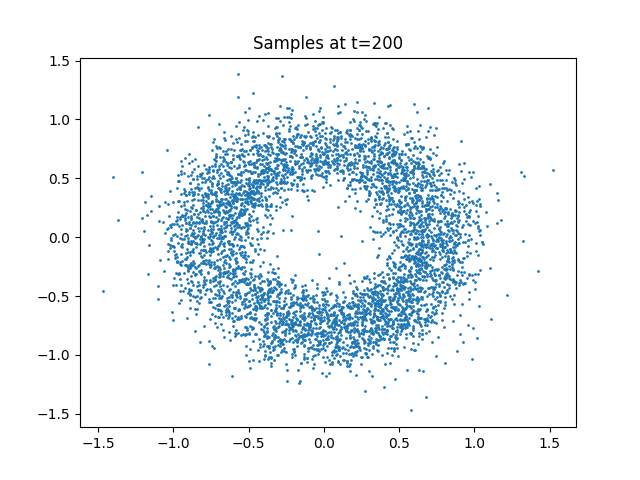
\includegraphics[width=0.3\textwidth]{exps/ddpm_2_200_0.0001_0.02_circles/samples_200.png} &
            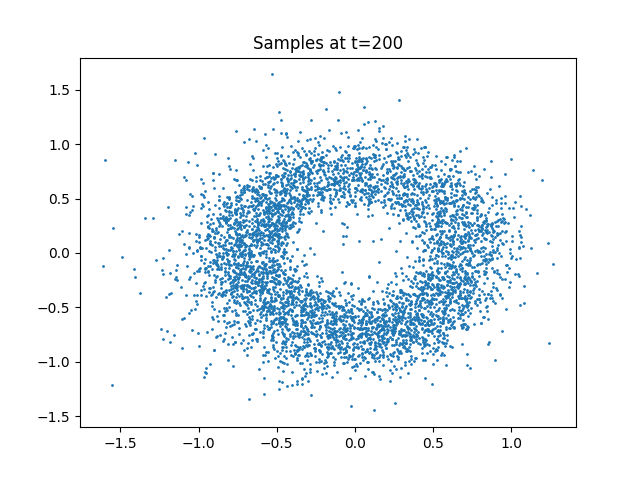
\includegraphics[width=0.3\textwidth]{exps/ddpm_2_200_0.001_0.2_circles/samples_200.png} &
            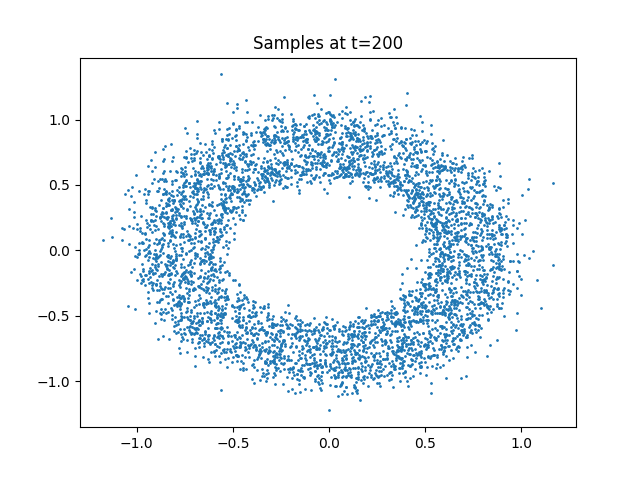
\includegraphics[width=0.3\textwidth]{exps/ddpm_2_200_1e-05_0.002_circles/samples_200.png} \\
            $\beta=1\text{e-}4\to0.02$ & $\beta=1\text{e-}3\to0.2$ & $\beta=1\text{e-}5\to0.002$ \\[0.5em]
            
            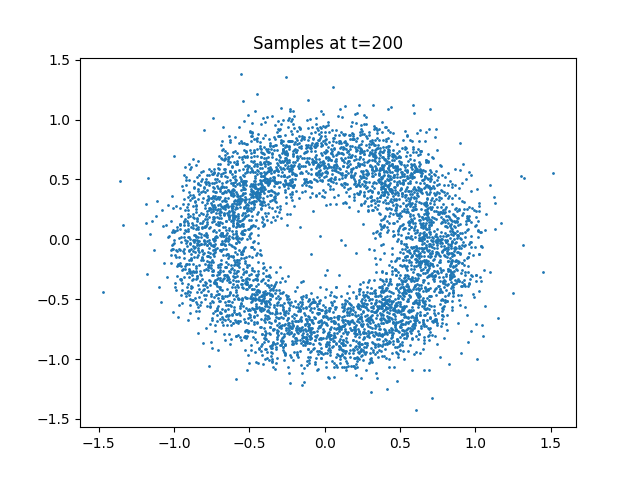
\includegraphics[width=0.3\textwidth]{exps/ddpm_2_200_1e-05_0.02_circles/samples_200.png} &
            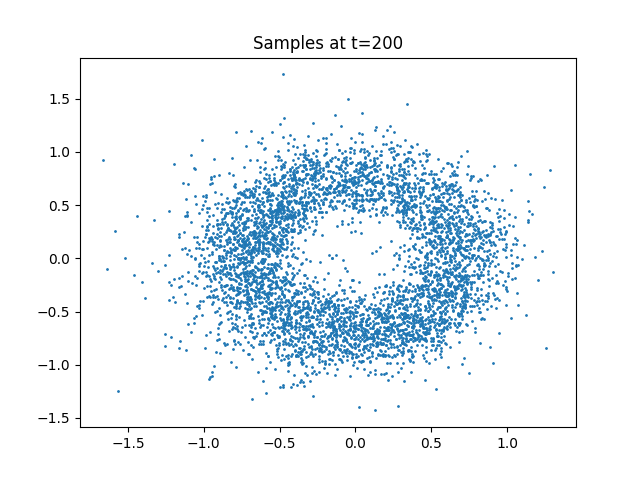
\includegraphics[width=0.3\textwidth]{exps/ddpm_2_200_0.0001_0.2_circles/samples_200.png} &
            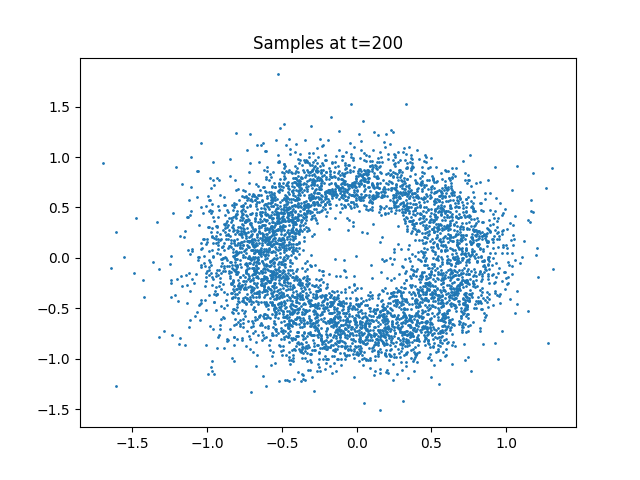
\includegraphics[width=0.3\textwidth]{exps/ddpm_2_200_1e-05_0.2_circles/samples_200.png} \\
            $\beta=1\text{e-}5\to0.02$ & $\beta=1\text{e-}4\to0.2$ & $\beta=1\text{e-}5\to0.2$ \\
        \end{tabular}
        \caption{Samples generated by DDPM with \textbf{varying beta schedules} for the Circles dataset.}
        \label{fig:beta_circles}
    \end{figure}

    \begin{figure}[ht]
        \centering
        \begin{tabular}{ccc}
            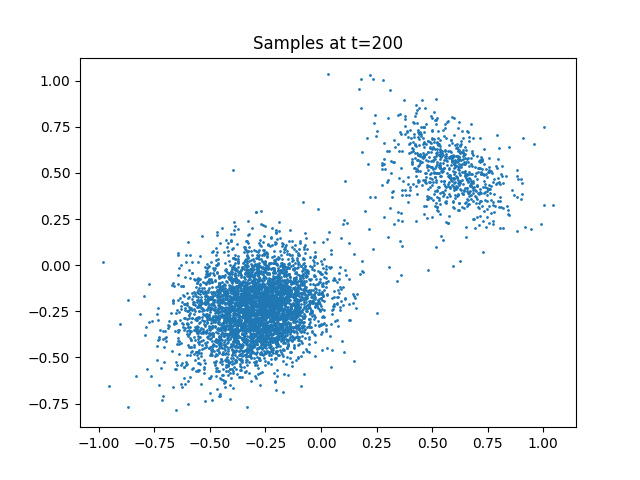
\includegraphics[width=0.3\textwidth]{exps/ddpm_2_200_0.0001_0.02_blobs/samples_200.png} &
            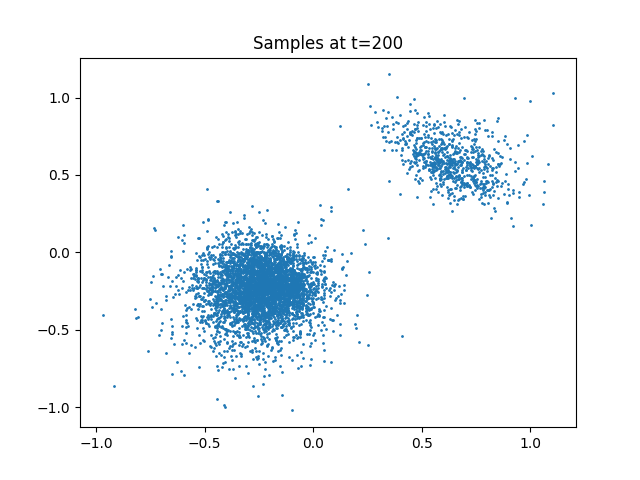
\includegraphics[width=0.3\textwidth]{exps/ddpm_2_200_0.001_0.2_blobs/samples_200.png} &
            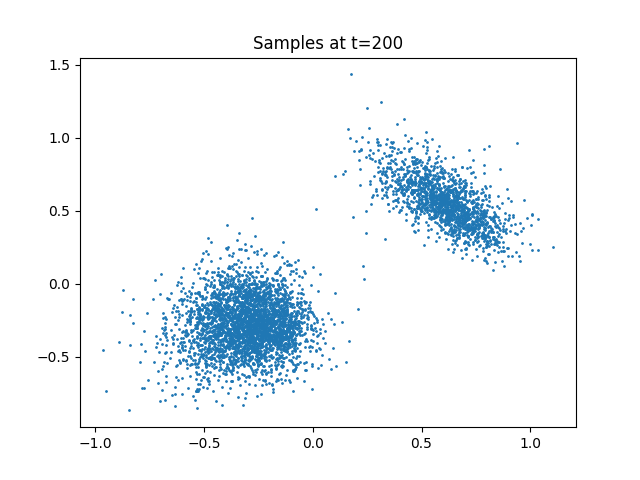
\includegraphics[width=0.3\textwidth]{exps/ddpm_2_200_1e-05_0.002_blobs/samples_200.png} \\
            $\beta=1\text{e-}4\to0.02$ & $\beta=1\text{e-}3\to0.2$ & $\beta=1\text{e-}5\to0.002$ \\[0.5em]
            
            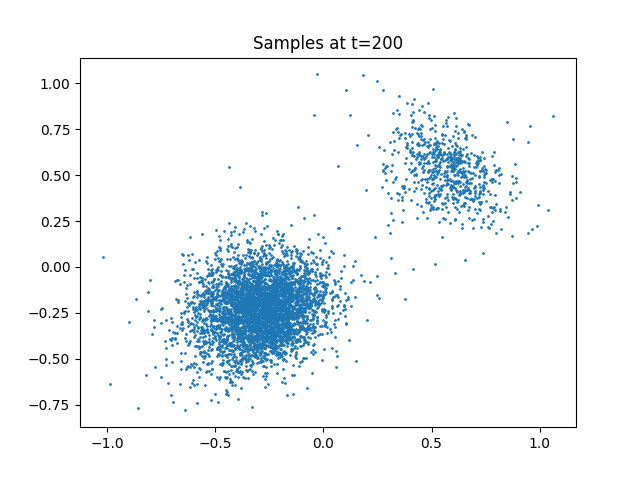
\includegraphics[width=0.3\textwidth]{exps/ddpm_2_200_1e-05_0.02_blobs/samples_200.png} &
            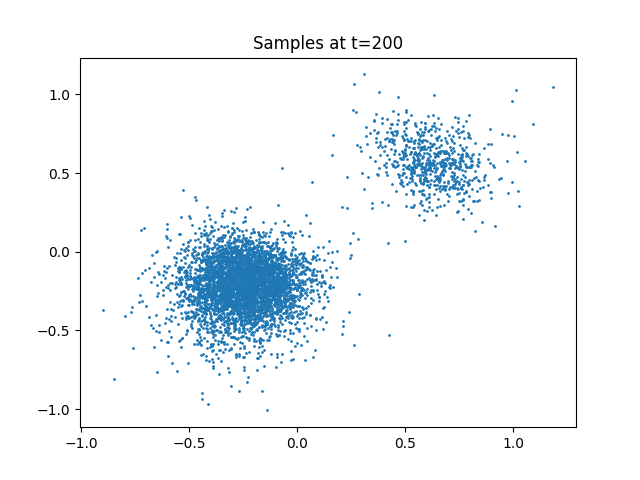
\includegraphics[width=0.3\textwidth]{exps/ddpm_2_200_0.0001_0.2_blobs/samples_200.png} &
            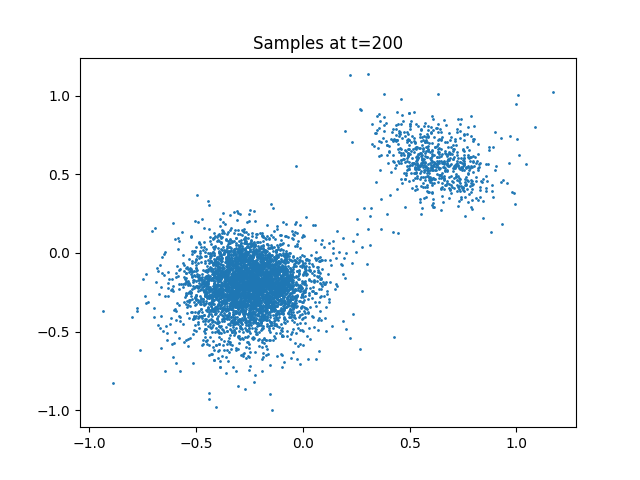
\includegraphics[width=0.3\textwidth]{exps/ddpm_2_200_1e-05_0.2_blobs/samples_200.png} \\
            $\beta=1\text{e-}5\to0.02$ & $\beta=1\text{e-}4\to0.2$ & $\beta=1\text{e-}5\to0.2$ \\
        \end{tabular}
        \caption{Samples generated by DDPM with \textbf{varying beta schedules} for the Blobs dataset.}
        \label{fig:beta_blobs}
    \end{figure}

    \begin{figure}[ht]
        \centering
        \begin{tabular}{ccc}
            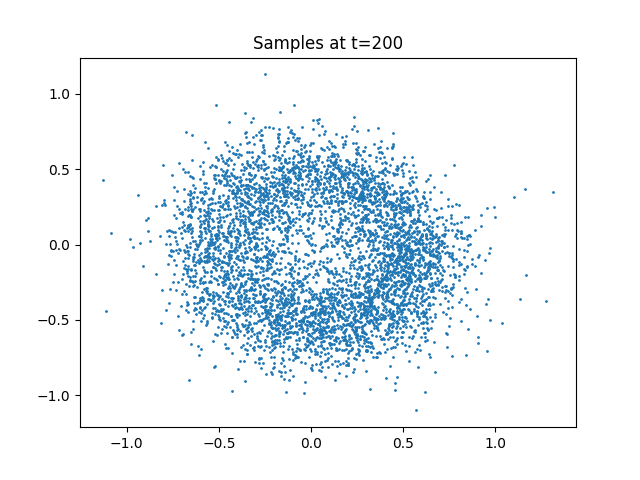
\includegraphics[width=0.3\textwidth]{exps/ddpm_2_200_0.0001_0.02_manycircles/samples_200.png} &
            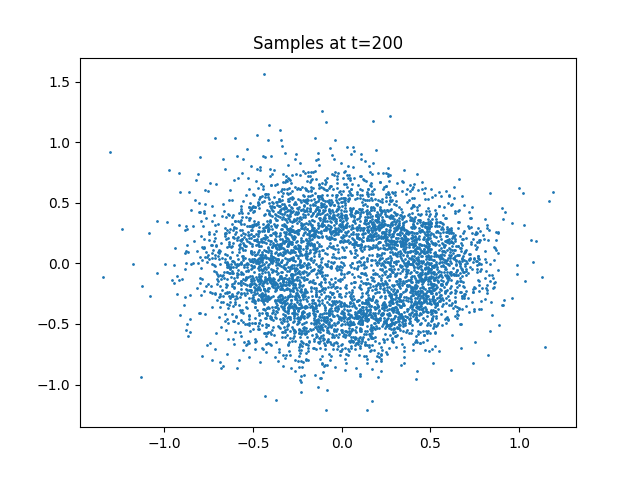
\includegraphics[width=0.3\textwidth]{exps/ddpm_2_200_0.001_0.2_manycircles/samples_200.png} &
            \includegraphics[width=0.3\textwidth]{exps/ddpm_2_200_1e-05_0.002_manycircles/samples_200.png} \\
            $\beta=1\text{e-}4\to0.02$ & $\beta=1\text{e-}3\to0.2$ & $\beta=1\text{e-}5\to0.002$ \\[0.5em]
            
            \includegraphics[width=0.3\textwidth]{exps/ddpm_2_200_1e-05_0.02_manycircles/samples_200.png} &
            \includegraphics[width=0.3\textwidth]{exps/ddpm_2_200_0.0001_0.2_manycircles/samples_200.png} &
            \includegraphics[width=0.3\textwidth]{exps/ddpm_2_200_1e-05_0.2_manycircles/samples_200.png} \\
            $\beta=1\text{e-}5\to0.02$ & $\beta=1\text{e-}4\to0.2$ & $\beta=1\text{e-}5\to0.2$ \\
        \end{tabular}
        \caption{Samples generated by DDPM with \textbf{varying beta schedules} for the Manycircles dataset.}
        \label{fig:beta_manycircles}
    \end{figure}

    \begin{figure}[ht]
        \centering
        \begin{tabular}{ccc}
            \includegraphics[width=0.3\textwidth]{exps/ddpm_3_200_0.0001_0.02_helix/samples_200.png} &
            \includegraphics[width=0.3\textwidth]{exps/ddpm_3_200_0.001_0.2_helix/samples_200.png} &
            \includegraphics[width=0.3\textwidth]{exps/ddpm_3_200_1e-05_0.002_helix/samples_200.png} \\
            $\beta=1\text{e-}4\to0.02$ & $\beta=1\text{e-}3\to0.2$ & $\beta=1\text{e-}5\to0.002$ \\[0.5em]
            
            \includegraphics[width=0.3\textwidth]{exps/ddpm_3_200_1e-05_0.02_helix/samples_200.png} &
            \includegraphics[width=0.3\textwidth]{exps/ddpm_3_200_0.0001_0.2_helix/samples_200.png} &
            \includegraphics[width=0.3\textwidth]{exps/ddpm_3_200_1e-05_0.2_helix/samples_200.png} \\
            $\beta=1\text{e-}5\to0.02$ & $\beta=1\text{e-}4\to0.2$ & $\beta=1\text{e-}5\to0.2$ \\
        \end{tabular}
        \caption{Samples generated by DDPM with \textbf{varying beta schedules} for the Helix dataset.}
        \label{fig:beta_helix}
    \end{figure}

% \section*{Acknowledgements}



\end{document}